\documentclass[conference]{IEEEtran}
\usepackage[english]{babel}
\usepackage{multicol}
\usepackage{multirow}
\usepackage{url,hyperref,graphicx,float,times}
%\usepackage{sectsty}
%\usepackage{authblk}
\usepackage{textcomp}
\usepackage{cite}
% \graphicspath{{../pdf/}{../jpeg/}}
% \DeclareGraphicsExtensions{.pdf,.jpeg,.png}
\usepackage[caption=false,font=footnotesize]{subfig}

\usepackage{url}

\begin{document}

\title{An Empirical Measurement-Based Analysis for Linux-based Real-Time Multiprocessor Scheduling}

\author{\IEEEauthorblockN{Ching-Chun (Jim) Huang} \IEEEauthorblockA{Department of\\Computer Science and Information
Engineering\\National Cheng Kung University, Taiwan\\ No.1, University Road, Tainan City 701, Taiwan (R.O.C.)}
\and \IEEEauthorblockN{Chung-Fan Yang} \IEEEauthorblockA{Department of Electrical Engineering\\
National Cheng Kung University, Taiwan\\ No.1, University Road, Tainan City 701, Taiwan (R.O.C.)}}

\maketitle

\begin{abstract}
A real-time, Linux-based testbed, which we have developed for empirically evaluating multiprocessor
scheduling hehavior is presented, along with various enhancements that remove some of the fundamental
barriers to eliminate potential latency. Both raw performance and schedulability are considered for
hard real-time constraints. To our knowledge, this paper is the first attempt by anyone to obtain
comprehensive performance results regarding the scheduler and its interaction with external events.
\end{abstract}

\section{Introduction}

The processing of time-critical tasks, depends upon the capacity of the system to respond to an event, within
a known and bounded interval of time. We have constructed a set of system utilities as a testbed to discover
Linux scheduling, multi-core overhead and real-time performance from microscopic view.

The landscape in terms of hardware platforms has been changing: "server-class" multiprocessor machines have
been available for some time now, and SoC vendors are shifting to multi-core technologies as real-time system
solutions. Our goal was to produce a platform that supports both static and dynamic workloads for real-time constraints.

\section{Related Work}

It has been more than 10 years since Linux engineers collaborate on the in-kernel real-time development, real-time
preemption or PREEMPT\textunderscore RT \cite{rt-linux}. The preemption latency of Linux kernel has been reduced by
one to several orders of magnitude, allowing it to compete commercial real-time operating systems.

Another relevant Linux-related prior effort is work by Calandrino \textit{et al}. \cite{Lozi:2016:LSD:2901318.2901326},
who built new tools that check for violation of the invariant online and visualize scheduling activity while analyzing
performance degradation for synchronization-heavy application on Linux.

\section{Methodology}

    The Completely Fair Scheduler (CFS) is a process scheduler which was merged into the 2.6.23 release of Linux kernel
    and is the default scheduler with O(1) complexity on selecting next task, giving static latency. In other words, parts
    of latency source of a Linux-based real-time system can be determined, at least for scheduler duration, shown in
    Figure \ref{fig:latency_timeline}.

    A new tool to visualize scheduling visualize is developed, enabling developers to record the scheduler states
    including executing process ID (PID), PID in scheduler run-queue, context switch points, timer interrupt execution,
    scheduling events, etc. on per processor core basis. It differs from profiling based methodology tools, e.g.
    perf \cite{perf}, by means of high fidelity and full-profiling fashion of the target system. It gathers entire
    activities inside Linux kernel in microsecond scale, being able to capture the impact of occasional short-burst
    scheduler events, which only last less that 10us. These events are mostly not shown in the result of sampling based
    measurement which focus on average-case execution time. By analyzing full-detailed record, we can not only
    capture the worst-case execution time (WCET), but also understand the cause of these incidents.

    Moreover, the behavior and characteristic of typical work-load used in the past, such as hackbench and stress \cite{rt-tests},
    are far from the real-world real-time applications. In result of this frustration, we also created a testing framework
    hosting a set of algorithms which resembled a real-time robot control system execution behavior, named after "mctest".
    It has the ability to be compiled either as user-space program or kernel module, that would give the insight of system-call
    and user-space I/O overhead, which is eliminated in kernel module expectedly.

    In addition, mctest would do a series of identically executions and record the execution time of each turn. These records
    can be used to determined the execution jitter of the application on the real-time system, which besides wakeup latency.
    This could be used to reflect to the system-call overhead of the system. We have been utilizing mctest as the testing
    work-load and jitter measurement tool during methodology.

    \begin{figure} \centering \includegraphics[width=3.5in]{img/latency_timeline.png} \caption{Task Wake-up Latency}
    \label{fig:latency_timeline} \end{figure}

\section{Experiment}

    We performed multiple experiments on 2 ARM Cortex-A9 based boards, shown in Table \ref{hardware_list}, widely adopted by industrial
    automation applications. Each test runs Linux kernel version 4.4 and PREEMPT\textunderscore RT \cite{preemptrt} with
    minimal root file system.

    \begin{table*}[]
        \centering \caption{Experiment Platforms}
        \label{hardware_list}
	\begin{tabular}{|l|c|c|} \hline Platform Name & Altera
        Cyclone V Development Kit & NXP i.MX6 Sabre \\ \hline Processor & 2x ARM Cortex-A9 & 4x ARM Cortex-A9 \\
        \hline Memory & 1 GB & 1 GB \\ \hline Additional configuration & None & \begin{tabular}[c]{@{}c@{}}L2 Cache
        locked down to CPU1,\\ Isolated CPU1,\\ Enabled tickless on CPU1 \\ Real-time task pinned to CPU1 \end{tabular}
    \\ \hline \end{tabular} \end{table*}

    Our experiment begins with known tuning practices which includes processor isolation \cite{isolatedcpu}, tickless
    feature of kernel \cite{tickless}, L2 cache lockdown. We compared the measurement result of mctest with and without
    these tuning techniques on NXP i.MX6 Sabre platform. Measurement results are shown in
    Figure \ref{fig:imx6_mctest_v}, \ref{fig:imx6_mctest_iso}, and \ref{fig:imx6_mctest_lock}, verifying the effectiveness of
    these known tuning techniques and providing results as a baseline. We are able to see the WCET with and without
    tuning are 153us and 86us. This gives us the hint that the scheduling would harms the real-time performance. This
    scheduling overhead could be separated into 2 parts, scheduler overhead and cache contention on SMP system. With L2
    Cache lockdown we are able to mitigate most of the cache contention, but still resulting some degree of jitter about
    76us in maximum.

    \begin{figure} \centering \includegraphics[width=3in]{img/mctest-none.png} \caption{Mctest on i.MX6 Sabre}
    \label{fig:imx6_mctest_v} \end{figure}
    
    \begin{figure} \centering \includegraphics[width=3in]{img/mctest-iso.png} \caption{Mctest on i.MX6 Sabre with
    isolated cpu and tickless feature} \label{fig:imx6_mctest_iso} \end{figure}
    
    \begin{figure} \centering \includegraphics[width=3in]{img/mctest-lock.png} \caption{Mctest on i.MX6 Sabre with
    isolated cpu, tickless feature and L2 cached lockdown} \label{fig:imx6_mctest_lock} \end{figure}
    
    \subsection{Eliminate System Call Overhead}

    In addition, we compared the user-space mctest result with kernel space measurement, shown in figure
    \ref{fig:imx6_mctest_k_v} and \ref{fig:imx6_mctest_k_lock} with WCET of 27us and 17us. With these result, we are
    able to identify the sources of jitter are system calls. To mitigate these, we first proposed to rewrite real-time
    applications as kernel modules. But this is tedious and making the debugging process difficult. Thus, we proposed a
    second approach, Kernel Mode Linux(KML) \cite{KML} \cite{KMLConf}, allowing userspace programs running in kernel
    address space. Thus, system calls become jump instructions instead of instructions that traps the processor. Also,
    this would mitigate the cache contention while switching in and out the kernel during system call.
    In addition, we have wrapped system calls with vDSO \cite{vDSO} for better compatibility. It results in
    user-space program running in KML with WCET similar to Linux kernel module variants.

    \begin{figure} \centering \includegraphics[width=3in]{img/mctest-k-none.png} \caption{Kernel mctest on i.MX6 Sabre}
    \label{fig:imx6_mctest_k_v} \end{figure}
    
    \begin{figure} \centering \includegraphics[width=3in]{img/mctest-k-lock.png} \caption{Kernel mctest on i.MX6 Sabre
    with isolated cpu, tickless feature and L2 cached lockdown} \label{fig:imx6_mctest_k_lock} \end{figure}
    
\subsection{Scheduler Overhead Measurement}
    
    Identifying that scheduler is also a source of jitter, we applied our proposed scheduler profiling tool to evaluate
    and identify of which part of the scheduling process is the source of jitter. Knowing the IRQ latency, and
    context-switching latency, we would like to evaluate the scheduler duration. Traditionally, the latency of this part
    is considered static with the CFS algorithm complexity, designed to be O(1), but real measurement results are
    lacking. Thus, we set our proposed profiler to record the increment of scheduler run-queue and scheduler
    context-switching events with switched-to PID of each processors. A analyzer will process the recorded data and
    gives out the scheduler duration of a specified process, enabling us the understand the scheduling of real-time task
    in SMP system. The result of running a solo instance of cyclictest on Cyclone V Development Kit is shown in figure
    \ref{fig:sd_noload}. The latency could be considered static with maximum 17us. This result matches traditional
    considerations, but with the interference from other work-load, the jitter will start to emerge.

    \begin{figure} \centering 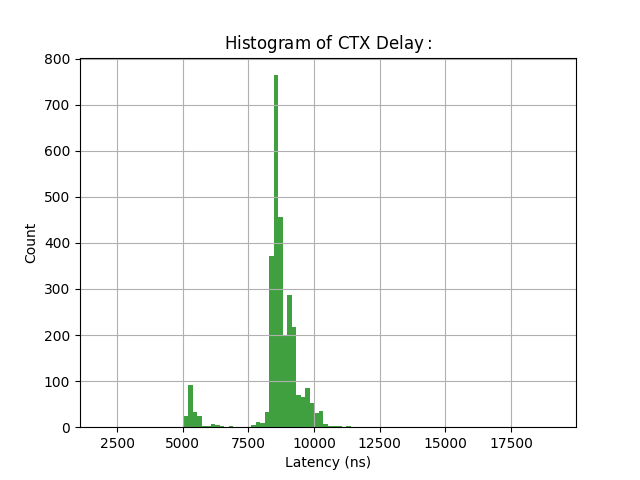
\includegraphics[width=3in]{img/sd-noload.png} \caption{Scheduler duration of solo
    cyclictest, no load} \label{fig:sd_noload} \end{figure}

\subsubsection{Scheduler Duration under Different Loading Condition}

    To measure the source of scheduler duration jitter, We created additional work-load, executing alone with
    cyclictest, with FIFO scheduling policy and highest priority in Cyclone V based system, during profiling session. We
    created a overloaded condition, which has 8 stress threads, doing either CPU, memory or I/O bounded task. The
    scheduler duration of cyclictest real-time task under each type of loading condition is shown in figure
    \ref{fig:sd_cpu}, \ref{fig:sd_memory}, and \ref{fig:sd_io}. This result exhibits a mostly static scheduler
    duration with seldom jitter with maximum of 20us in CPU and I/O bounded loads. But putting the system in to heavy
    memory loading condition, the result, shown in figure \ref{fig:sd_memory} shows an increased average of scheduler
    duration and exhibits random jitter up to 34us. The spread of distribution of scheduler duration would also become
    wilder. This informs us that the scheduler duration is not a static value and will increase alone with the system's
    load, especially memory related load. This informs that the scheduler runnable task selection process execution time
    could be lengthen by user-space task, doing memory bounded tasks.

    \begin{figure} \centering 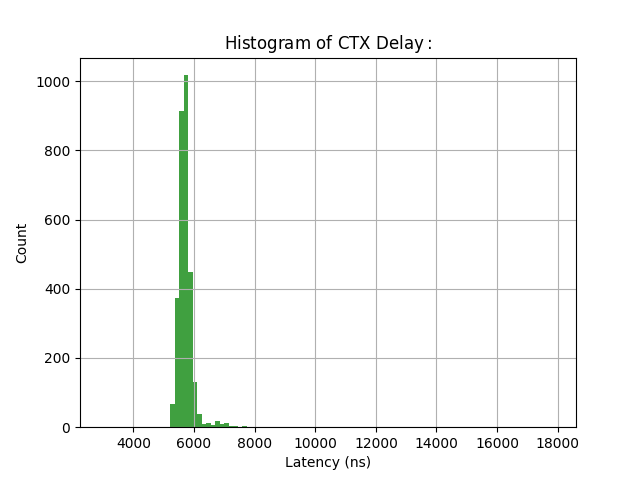
\includegraphics[width=3in]{img/sd-cpu.png} \caption{Scheduler duration of cyclictest
    with CPU bounded load} \label{fig:sd_cpu} \end{figure}

    \begin{figure} \centering 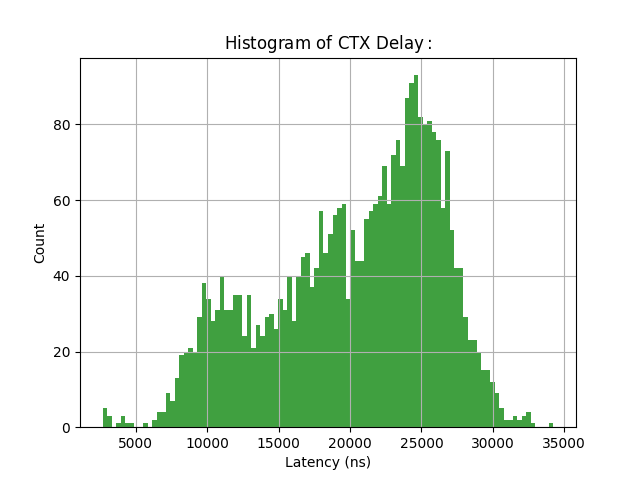
\includegraphics[width=3in]{img/sd-memory.png} \caption{Scheduler duration of cyclictest
    with memory bounded load} \label{fig:sd_memory} \end{figure}

    \begin{figure} \centering 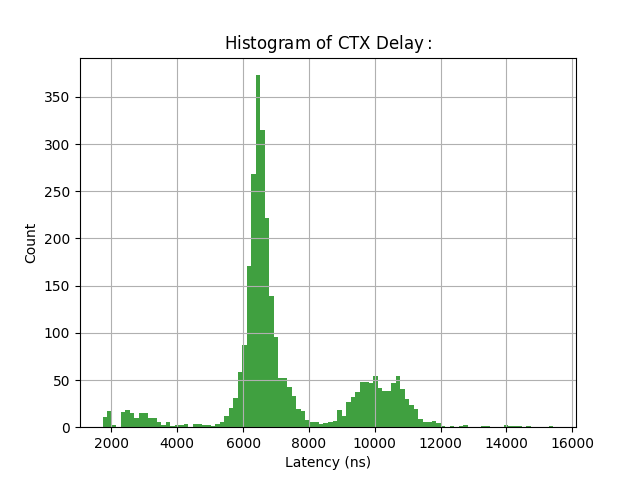
\includegraphics[width=3in]{img/sd-io.png} \caption{Scheduler duration distribution of
    cyclictest with I/O bounded load} \label{fig:sd_io} \end{figure}

    To mitigate the influence of memory bounded tasks, we isolated the real-time task into dedicated CPU core, and
    pinned memory bounded tasks to another CPU core. In addition, we make the shared L2 cache only accessible from the
    CPU core, running real-time task. The result of scheduler duration in shown in figure \ref{fig:sd_iso}. The
    scheduler duration is stabilized and showing as distribution as other loading conditions. The stress memory bounded
    tasks were designed to spin on malloc and free calls. This suggests us that memory allocation and deallocation would
    decrease the scheduler performance and increase its execution jitter via cache and memory model. Also, we gathered
    the result of pining both real-time and loads to same CPU core. Figure \ref{fig:sd_same_no_cache} shows the result
    of running on CPU core without L2 cache.  Comparing with figure \ref{fig:sd_memory}, result under 2 core SMP, this
    result showns a slight improvement of average latency and jitter. This informs that shared L2 cache and dynamic
    number of loading tasks, sharing CPU with real-time task, would be the source of scheduler duration jitter. Thus,
    decrease the use of dynamic memory allocation, real-time task CPU isolation and cache lockdown could prevent raising
    the scheduler duration, keeping it as a stable value, about 10us.

    \begin{figure} \centering 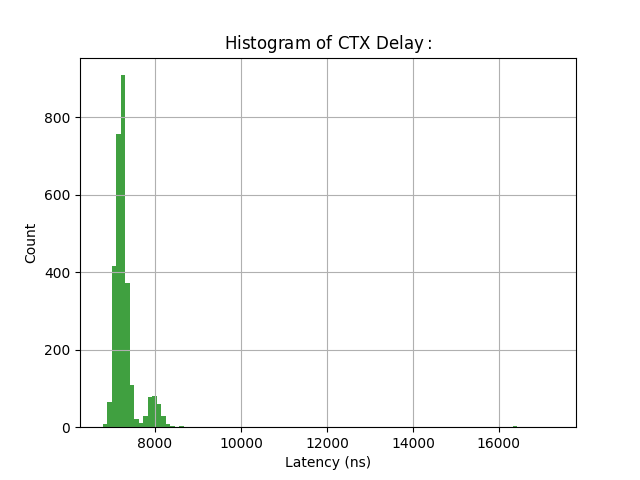
\includegraphics[width=3in]{img/sd-iso.png} \caption{Scheduler duration of cyclictest with
    memory bounded load on different cores} \label{fig:sd_iso} \end{figure}

    \begin{figure} \centering 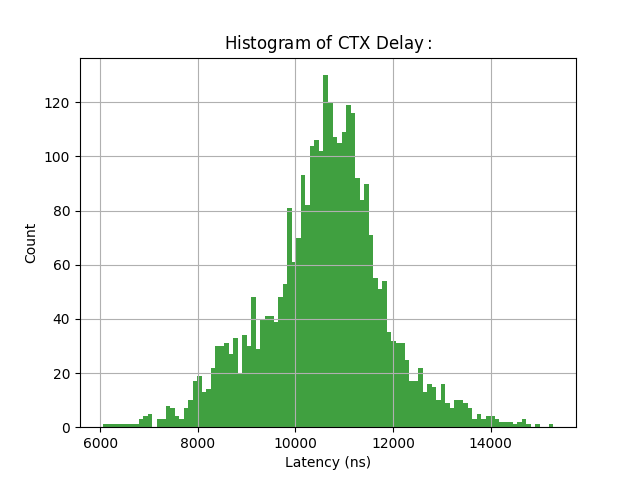
\includegraphics[width=3in]{img/sd-same-no-cache.png} \caption{Scheduler duration of
    cyclictest with memory bounded load on same core} \label{fig:sd_same_no_cache} \end{figure}

\section{Conclusion}
    We have evaluated Linux real-time behavior by profiling kernel scheduler and measuring the latency.
    An intensive interrupt load can cause long OS latencies due to the design of the interrupt
    processing mechanism. We proposed new tools to visualize task scheduling in fine-grained scale(microsecond level).
    It encourages us to focus on not only interrupt latency but also scheduler durations, lock, etc., andt would thus
    be highly desirable to combine existing techniques, e.g isolated CPU, tickless kernel, to improve task responsiveness
    under various target application characteristics, with our testbed.

\bibliographystyle{IEEEtran}
\bibliography{references}

\end{document}
